%%%%%%%%%%%%%%%%%%%%%%%%%%%%%%%%%%%%%%%%%%%%%%%%%%%%%%%%%%%%%%%%%%%%%%%%%%%%%
% FinGuard-AI / RT-IIPF -- IEEE JOURNAL manuscript (IEEEtran, journal class)
%
% This is the EXTENDED journal version of the conference draft
% (finguard.tex). Differences: journal document class, two additional
% experiments (threshold sensitivity, scorer substitution), expanded
% related work and discussion, and a deployment-recommendation section.
%
% Compile:  pdflatex finguard && pdflatex finguard
%
% ACTION ITEMS BEFORE SUBMISSION (marked \todo{} in text):
%   - author names, affiliations, emails
%   - conference name/dates in \IEEEoverridecommandlockouts block if required
%   - verify target journal's length and formatting requirements
%   - complete/verify all bibliography entries
%%%%%%%%%%%%%%%%%%%%%%%%%%%%%%%%%%%%%%%%%%%%%%%%%%%%%%%%%%%%%%%%%%%%%%%%%%%%%
\documentclass[journal]{IEEEtran}
\IEEEoverridecommandlockouts
\usepackage{cite}
\usepackage{amsmath,amssymb}
\usepackage{graphicx}
\usepackage{booktabs}
\usepackage{url}
\usepackage[hidelinks]{hyperref}
\usepackage{xcolor}
\newcommand{\todo}[1]{\textcolor{red}{[TODO: #1]}}

\begin{document}

\title{RT-IIPF: Real-Time Inline Interception of Fraudulent UPI Transactions
with Transactional Rollback and Unsupervised Anomaly Scoring}

\author{\todo{Author One},~\IEEEmembership{Student Member,~IEEE,}
        \todo{Author Two},~\IEEEmembership{Member,~IEEE}
\thanks{\todo{Authors are with the Department of ..., Institution, City,
India (e-mail: ...).}}
\thanks{Manuscript received \todo{date}; revised \todo{date}.}}

\maketitle

\begin{abstract}
Conventional payment-fraud analytics operate retrospectively: transactions
settle, logs are analysed downstream, and recovery is attempted after funds
have already moved. In high-velocity real-time rails such as India's Unified
Payments Interface (UPI), this latency renders recovery frequently
impossible. We present RT-IIPF, a working prototype that relocates the fraud
decision \emph{inside} the payment transaction boundary. The switch acquires
pessimistic locks on both ledger rows, applies the debit and credit
provisionally within an open ACID transaction, suspends the executing thread
pending a verdict from an isolated inference microservice, and then either
commits or aborts. A fraudulent transfer is rolled back atomically and never
attains durable existence, while the account lock and audit record survive
the rollback via an independent transaction. We evaluate the system on
250{,}000 UPI transactions. Because the public dataset's fraud labels are
statistically uninformative (ROC-AUC $\approx 0.48$ for every detector
tested), we adopt perturbation-based synthetic fraud injection with an
explicit negative control. Four findings are reported, including negative
ones. First, an ablation across enrichment layers shows that client
telemetry raises operating-point recall $22\times$ while \emph{lowering}
ROC-AUC, indicating that AUC is the wrong selection criterion under a
false-positive budget. Second, a threshold sweep establishes that the
deployed Isolation Forest admits no operating point that is simultaneously
effective and operationally tolerable. Third, substituting Local Outlier
Factor within the unchanged architecture raises recall from $0.147$ to
$0.745$ at identical false-positive cost while reducing inference latency
$3.3\times$, isolating scorer choice --- not the interception design --- as
the binding constraint; the velocity negative control survives the
substitution, establishing that blind spot as architectural rather than
model-dependent. Fourth, concurrency measurement falsifies the expected
hypothesis that lock-holding across the scoring hop limits throughput: the
constraint resides in the stateless inference tier, where four-way
replication yields $3.4$--$5.4\times$ speed-up. Single-client end-to-end
latency is 11--12\,ms. We conclude with a deployment recommendation derived
from these measurements.
\end{abstract}

\begin{IEEEkeywords}
fraud detection, anomaly detection, isolation forest, UPI, real-time
payments, microservices, ACID transactions, unsupervised learning
\end{IEEEkeywords}

%==============================================================
\section{Introduction}

The Unified Payments Interface processes billions of transactions monthly,
settling each in seconds. This velocity, which underpins UPI's utility, also
compresses the window available for fraud intervention to near zero. Once a
fraudulent transfer settles, funds are typically forwarded through
intermediary accounts and withdrawn before any retrospective analytic
pipeline raises an alert. The economics are asymmetric: detection accuracy
achieved after settlement contributes little if recovery is infeasible.

The dominant architectural pattern in deployed fraud analytics remains
post-facto: transaction logs are consumed by batch or streaming pipelines
that score transactions after they have committed, and flagged cases enter a
manual review or recovery workflow. We argue that for real-time rails the
decision must be relocated \emph{into} the transaction path, such that a
rejected payment is never durably recorded.

This paper describes RT-IIPF (Real-Time Inline Interception Payment
Framework), a functioning three-service prototype implementing this
relocation, together with an evaluation that is deliberate about reporting
negative results. Our contributions are:

\begin{enumerate}
\item \textbf{An inline interception mechanism} in which the fraud verdict
arbitrates an open database transaction, with a two-transaction pattern that
allows the security response (account lock, audit record) to survive the
ledger rollback it describes (Section~\ref{sec:arch}).

\item \textbf{A layered feature-enrichment design with an explicit trust
boundary}, in which client-supplied features are limited to those where
adversarial forgery increases rather than decreases anomaly, and decisive
temporal and demographic features are server-resolved
(Section~\ref{sec:enrich}).

\item \textbf{An evaluation methodology for unsupervised fraud scoring under
unreliable public labels}, using perturbation-based synthetic injection with
a negative control that quantifies an architectural blind spot rather than
concealing it (Section~\ref{sec:method}).

\item \textbf{Four measured findings, several of them negative}: the
inadequacy of ROC-AUC as a selection metric under false-positive budgets;
the absence of any tolerable operating point for the deployed scorer; the
decisive superiority of a density-based scorer substituted within the
unchanged architecture, together with the survival of the velocity blind
spot under that substitution; and the empirical falsification of our own
expected scaling bottleneck (Section~\ref{sec:results}).

\item \textbf{A deployment recommendation} derived from, rather than
asserted alongside, the measurements (Section~\ref{sec:deploy}).
\end{enumerate}

We explicitly do not claim that real-time transaction scoring is itself
novel; variants are known in industrial practice. Our contribution is an
open, reproducible, end-to-end prototype exhibiting the transactional
mechanics in full, accompanied by an honest characterisation of where such a
design succeeds and where it does not.

%==============================================================
\section{Related Work}

Isolation Forest~\cite{liu2008} detects anomalies by exploiting the
observation that outliers require fewer random axis-parallel partitions to
isolate than inliers, yielding linear time complexity and low memory
footprint --- properties attractive for latency-constrained inference. Local
Outlier Factor~\cite{breunig2000} instead assigns a degree of outlierness by
comparing local reachability densities, and One-Class SVM~\cite{scholkopf2001}
estimates a support region enclosing the normal class. Comparative studies of
unsupervised outlier detectors~\cite{campos2016} report substantial
task-dependent variation in relative ranking, motivating empirical baseline
comparison rather than a priori model selection.

Surveys of financial fraud detection~\cite{abdallah2016,adewumi2017} document
the field's predominant reliance on supervised learning over labelled
historical fraud, and note the recurring obstacles of extreme class
imbalance, label latency, and concept drift. These obstacles motivate
unsupervised formulations, which require no fraud labels and can in principle
respond to novel attack patterns absent from historical data.

\todo{Add 2--4 citations specific to UPI or Indian real-time payment
security, and one on transactional/ACID guarantees in payment switches, to
strengthen venue fit.}

%==============================================================
\section{System Architecture}
\label{sec:arch}

\subsection{Service decomposition}

RT-IIPF comprises three processes communicating over HTTP/JSON: a React
client presenting the payment interface and an operational monitor; a Spring
Boot~3 switch (Java~21) owning authentication, the ledger, and transactional
control; and a FastAPI inference node (Python~3) exposing a single scoring
endpoint. The ledger is an embedded H2 relational database accessed through
Spring Data JPA, comprising \texttt{users}, \texttt{balances}, and
\texttt{transaction\_logs}.

\subsection{The interception pipeline}

On receipt of a payment request the switch executes the following within one
\texttt{@Transactional} method:

\begin{enumerate}
\item Resolve payer and payee by virtual payment address; reject locked
accounts; verify the MPIN digest in constant time.
\item Acquire \texttt{PESSIMISTIC\_WRITE} locks on both balance rows, always
in ascending account-identifier order so that opposing concurrent payments
cannot deadlock.
\item Apply the debit and credit to the persistence context. These changes
are real but uncommitted --- the transaction exists provisionally.
\item Issue a synchronous HTTP request to the inference node carrying the
assembled feature vector, blocking the request thread. Connect and read
timeouts are bounded (300\,ms, 1500\,ms) because ledger locks are held for
the duration.
\item Branch on the returned verdict.
\end{enumerate}

\subsection{Rollback with surviving audit}

A verdict of fraud creates an apparent contradiction: the ledger movement
must be erased, yet the institution must durably record the attempt and
immobilise the account. Naively writing both inside the payment transaction
would destroy the audit record along with the movement.

RT-IIPF resolves this with a two-transaction pattern. The account lock and
the \texttt{BLOCKED\_FRAUD} audit row are written by a component annotated
\texttt{Propagation.REQUIRES\_NEW}, which suspends the payment transaction,
commits independently, and returns. Only then does the payment path throw
\texttt{FraudulentTransactionException}; the framework marks the suspended
transaction rollback-only and the provisional debit and credit are discarded
atomically. The commit path is simply the absence of this exception. The
observable postcondition of a blocked payment is therefore: balances
unchanged, account locked, audit row present.

\subsection{Fail-closed availability posture}

If the inference node is unreachable or exceeds its timeout, the switch
rejects the payment (HTTP 503) rather than admitting it unscored. Safety is
preferred to availability; Section~\ref{sec:limits} discusses the cost.

%==============================================================
\section{Feature Enrichment and Trust Boundary}
\label{sec:enrich}

The client interface collects six fields, of which three reach the model
(amount, transaction type, merchant category); the two addresses serve as
routing keys and the MPIN as an authentication secret that never leaves the
switch. The model receives thirteen features, assembled in three layers:

\begin{itemize}
\item \textbf{L1 --- user-entered} (3 features): amount, transaction type,
merchant category.
\item \textbf{L2 --- client telemetry} (2 features): device class and network
type, captured autonomously by the client at page load without user
interaction.
\item \textbf{L3 --- server enrichment} (8 features): counterparty age
bands, sender state, both issuing banks, resolved from the account database;
and hour, weekday, and weekend flag, resolved from the switch's own clock.
\end{itemize}

Enrichment imposes negligible latency because both account rows are already
materialised for authentication and routing; no additional query is issued.

The partition is a deliberate trust boundary. Features an adversary controls
are those for which anomalous values \emph{increase} the anomaly score, so
misreporting is self-defeating. Features that would most benefit an
adversary --- transacting at a plausible hour, presenting a normal
demographic profile --- are resolved server-side and are not client-assertable.

%==============================================================
\section{Evaluation Methodology}
\label{sec:method}

\subsection{Motivation for synthetic injection}

The evaluation corpus comprises 250{,}000 UPI transactions with seventeen
attributes, split 80/20 into training and held-out sets. The corpus carries a
\texttt{fraud\_flag} annotation, which we found to be statistically
uninformative: no detector evaluated in this work, supervised or
unsupervised, exceeded ROC-AUC $0.48$ against it, a value consistent with
random assignment. Reporting accuracy against such labels would be vacuous.

We therefore adopt perturbation-based synthetic injection. Four fraud
archetypes are instantiated by sampling genuine held-out transactions and
overwriting only the attributes that define each archetype, leaving all
remaining attributes at realistic sampled values so that synthetics are not
trivially separable by marginal inspection. One hundred vectors per
archetype (400 total) are injected into 50{,}000 clean held-out
transactions, yielding $0.79\%$ synthetic prevalence.

\subsection{Archetypes and the negative control}

\begin{itemize}
\item \textbf{A --- off-hour high-value drain}: INR~25{,}000--60{,}000,
01:00--04:00, peer-to-peer, web origin.
\item \textbf{B --- velocity spike (negative control)}:
INR~2{,}000--6{,}000, business hours, common device and network. Each
constituent transfer is individually unremarkable; the attack exists only in
aggregate.
\item \textbf{C --- category anomaly}: INR~50{,}000--100{,}000 under an
everyday merchant category, daytime.
\item \textbf{D --- context anomaly}: INR~2{,}000--9{,}000, 00:00--04:00,
web and Wi-Fi origin.
\end{itemize}

Archetype~B is included as a negative control. The deployed model scores each
transaction independently and receives no velocity features; it is therefore
\emph{expected} to detect none of these vectors. Including B quantifies a
known architectural boundary instead of selecting archetypes favourable to
the system.

\subsection{Experimental configuration}

All experiments use seed~42 and are reproducible from the released
evaluation script. The deployed configuration is an Isolation Forest of 200
estimators with contamination $0.002$; raw scores are mapped to $[0,1]$ by
min--max normalisation whose upper bound is winsorised at the $99.95$th
percentile of the training score distribution, preventing a single extremal
training point from compressing the operational range. The production
threshold $\tau = 0.85$ was chosen to bound empirical false-positive rate
below $1\%$. Score-based baselines are compared at an equal $1\%$
false-positive budget, reflecting the operational reality that an inline
blocker is FPR-constrained rather than accuracy-constrained.

%==============================================================
\section{Results}
\label{sec:results}

\subsection{Detection under injection}

\begin{table}[t]
\caption{Detection by archetype at the production operating point
($\tau=0.85$), $n=100$ per archetype}
\label{tab:arch}
\centering
\begin{tabular}{llcc}
\toprule
& \textbf{Archetype} & \textbf{Mean score} & \textbf{Recall} \\
\midrule
A & Off-hour high-value drain & 0.781 & 0.26 \\
B & Velocity spike \emph{(neg.\ control)} & 0.350 & 0.00 \\
C & Category anomaly & 0.567 & 0.07 \\
D & Context anomaly & 0.799 & 0.26 \\
\midrule
\multicolumn{2}{l}{Clean held-out traffic ($n=50{,}000$)} &
\multicolumn{2}{c}{FPR $=0.0086$} \\
\bottomrule
\end{tabular}
\end{table}

Table~\ref{tab:arch} reports detection by archetype. Overall precision is
$0.121$, recall $0.148$, $F_1$ $0.133$, at ROC-AUC $0.723$ and a
false-positive rate of $0.86\%$.

\begin{figure}[t]
\centering
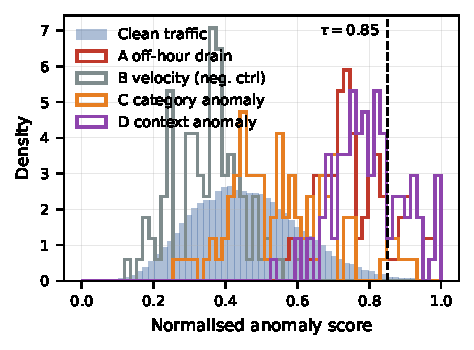
\includegraphics[width=\columnwidth]{figs/fig1_score_distributions.pdf}
\caption{Score distributions of clean traffic and each injected archetype.
Archetypes A and D concentrate immediately \emph{below} the production
threshold, visualising isolation saturation; the velocity negative control
(B) lies inside the clean distribution, confirming that a per-transaction
scorer cannot separate it.}
\label{fig:dists}
\end{figure}

Two failure mechanisms are identifiable, both visible in
Fig.~\ref{fig:dists}. First, \emph{isolation saturation}: amounts beyond the
training maximum cannot deepen an isolation path further, so archetypes
defined principally by extremal amount (A, C) asymptote below $\tau$ despite
being conspicuous to inspection --- their mass accumulates immediately below
the threshold rather than crossing it. Second, the velocity blind spot is
total, exactly as the negative control predicted: distribution B is
indistinguishable from clean traffic.

\subsection{Ablation of enrichment layers}

\begin{table}[t]
\caption{Enrichment-layer ablation; each layer independently trained and
calibrated}
\label{tab:ablation}
\centering
\begin{tabular}{lcccc}
\toprule
\textbf{Layer} & \textbf{Feat.} & \textbf{ROC-AUC} &
\textbf{Recall@$\tau$} & \textbf{Recall D} \\
\midrule
L1 form only        & 3  & \textbf{0.860} & 0.010 & 0.00 \\
L2 $+$ telemetry    & 5  & 0.747 & \textbf{0.228} & \textbf{0.40} \\
L3 $+$ server enr.  & 13 & 0.723 & 0.148 & 0.26 \\
\bottomrule
\end{tabular}
\end{table}

Table~\ref{tab:ablation} exhibits a dissociation between ranking quality and
operating-point utility. The form-only model attains the \emph{highest}
ROC-AUC ($0.860$), its ranking dominated by the amount marginal, yet it is
operationally inert: it detects $1\%$ of attacks at the deployable threshold
and none of archetype~D. Adding client telemetry sacrifices global AUC
($0.747$) while multiplying operating-point recall twenty-two-fold
($0.010 \rightarrow 0.228$) and enabling context-anomaly detection entirely
absent at L1 ($0.00 \rightarrow 0.40$).

Two conclusions follow. Enrichment features determine \emph{which attack
classes are detectable at all} under a fixed false-positive budget; and
ROC-AUC, which integrates over operating points that an inline blocker can
never adopt, is a misleading model-selection criterion for this task.
Recall at the deployed threshold is the decision-relevant metric.

\subsection{Baseline comparison}

\begin{table}[t]
\caption{Baselines at an equal $1\%$ false-positive budget}
\label{tab:baselines}
\centering
\begin{tabular}{lcccc}
\toprule
\textbf{Detector} & \textbf{AUC} & \textbf{Recall} &
\textbf{Prec.} & \textbf{$F_1$} \\
\midrule
Static rules            & ---   & 0.658 & 0.305 & 0.417 \\
Local Outlier Factor    & \textbf{0.896} & \textbf{0.745} &
\textbf{0.373} & \textbf{0.497} \\
One-Class SVM           & 0.783 & 0.675 & 0.351 & 0.462 \\
Isolation Forest (depl.)& 0.723 & 0.163 & ---   & ---   \\
\bottomrule
\end{tabular}
\end{table}

\begin{figure}[t]
\centering
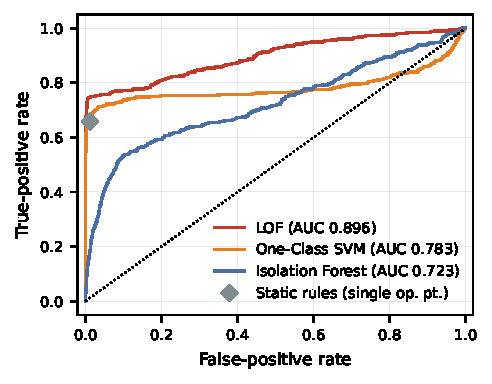
\includegraphics[width=\columnwidth]{figs/fig2_roc_comparison.pdf}
\caption{ROC comparison on the injected set. The rule baseline emits a
binary decision rather than a ranking and is therefore shown as its single
operating point; deriving a continuous pseudo-score for it would be
amount-dominated and hence near-oracular for the amount-defined archetypes,
an artefact of archetype construction rather than a property of the
classifier.}
\label{fig:roc}
\end{figure}

Table~\ref{tab:baselines} and Fig.~\ref{fig:roc} report a negative result
for the deployed model. Local Outlier Factor substantially outperforms
Isolation Forest (recall $0.745$ vs.\ $0.163$), as do One-Class SVM and even
static amount-and-hour rules. We attribute the deficit to Isolation Forest's
known degradation on sparse one-hot encoded categorical spaces, where
axis-parallel splits dilute the informative numeric dimensions, compounded
by the saturation effect of Section~VI-A.

We report this deliberately. It establishes that the architectural
contribution of RT-IIPF --- inline interception with transactional rollback
--- is orthogonal to, and presently bottlenecked by, the choice of scoring
model. The interception mechanism is model-agnostic; substituting a
density-based scorer is an immediate and well-characterised uplift path.

\subsection{Threshold sensitivity and the absence of a tolerable operating
point}

\begin{table}[t]
\caption{Threshold sensitivity of the deployed scorer. The rightmost column
expresses the false-positive rate operationally: genuine customers blocked
and locked out per 100{,}000 legitimate transactions.}
\label{tab:sweep}
\centering
\begin{tabular}{ccccc}
\toprule
$\tau$ & \textbf{Recall} & \textbf{FPR} & \textbf{Precision} &
\textbf{Blocked/100k} \\
\midrule
0.60 & 0.583 & 0.1771 & 0.026 & 17{,}710 \\
0.65 & 0.537 & 0.1101 & 0.038 & 11{,}012 \\
0.70 & 0.450 & 0.0638 & 0.053 & 6{,}380 \\
0.75 & 0.325 & 0.0357 & 0.068 & 3{,}574 \\
0.80 & 0.237 & 0.0181 & 0.095 & 1{,}808 \\
\textbf{0.85} & \textbf{0.147} & \textbf{0.0086} & \textbf{0.121} &
\textbf{858} \\
0.90 & 0.098 & 0.0041 & 0.159 & 412 \\
0.95 & 0.037 & 0.0015 & 0.169 & 148 \\
0.99 & 0.020 & 0.0006 & 0.222 & 56 \\
\bottomrule
\end{tabular}
\end{table}

\begin{figure}[t]
\centering
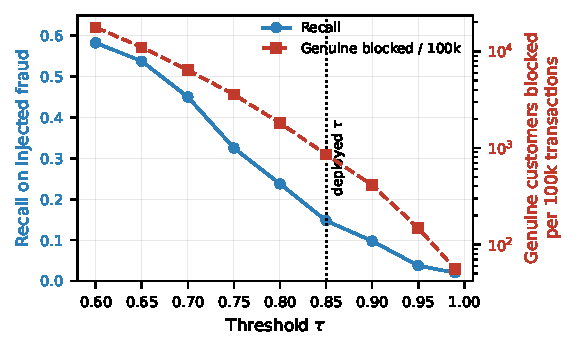
\includegraphics[width=\columnwidth]{figs/fig4_threshold_sensitivity.pdf}
\caption{Threshold sensitivity. Recall and genuine-customer block rate move
together across the entire sweep; no threshold yields both acceptable
detection and an operationally tolerable block rate.}
\label{fig:sweep}
\end{figure}

A threshold chosen by assertion invites the objection that a different
choice would produce different conclusions. Table~\ref{tab:sweep} and
Fig.~\ref{fig:sweep} sweep $\tau$ across $[0.60, 0.99]$.

The result is unfavourable to the deployed scorer, and we state it plainly:
\emph{no operating point is simultaneously effective and operationally
tolerable}. Reaching $45\%$ recall requires $\tau = 0.70$, which blocks
$6{,}380$ genuine customers per $100{,}000$ transactions --- at UPI's
national volume, an untenable rate of customer lockout. Conversely, the
deployed $\tau = 0.85$, chosen to hold false positives under $1\%$, admits
$85\%$ of injected attacks. Precision never exceeds $0.222$ anywhere in the
sweep.

This is not a tuning deficiency but a separability deficiency: the score
distributions of genuine and injected traffic overlap too heavily for any
single cut to divide them well (cf. Fig.~\ref{fig:dists}). The remedy must
therefore be a better scorer or richer features, not a better threshold ---
a conclusion the next subsection tests directly.

\subsection{Scorer substitution within the same architecture}

\begin{figure}[t]
\centering
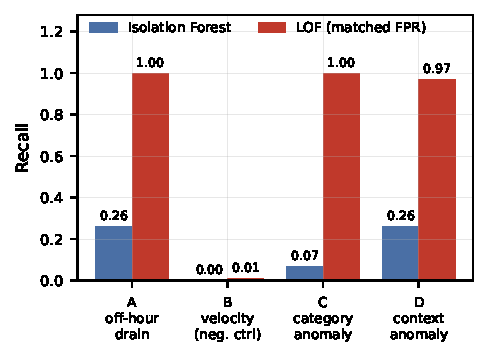
\includegraphics[width=\columnwidth]{figs/fig5_scorer_substitution.pdf}
\caption{Per-archetype recall at matched false-positive rate
($\mathrm{FPR}=0.0086$). Substituting LOF for the Isolation Forest resolves
archetypes A, C, and D almost completely at identical operational cost,
while archetype B remains undetected by both --- confirming that the
velocity blind spot is architectural rather than model-dependent.}
\label{fig:sub}
\end{figure}

Section~VI-C established that LOF ranks better than the deployed forest. A
ranking advantage does not by itself establish that the deployed system
would improve, because the two scorers are calibrated differently and the
architecture imposes latency and memory constraints. We therefore
substituted LOF into the full pipeline under the identical winsorised
calibration convention, and selected its threshold to match the deployed
model's measured false-positive rate exactly ($0.0086$), so that recall is
compared at equal operational cost.

The improvement is decisive: overall recall rises from $0.147$ to $0.745$.
Fig.~\ref{fig:sub} decomposes this by archetype. LOF detects the off-hour
drain (A) and category anomaly (C) archetypes completely ($1.00$), and the
context anomaly (D) nearly so ($0.97$), against $0.26$, $0.07$, and $0.26$
respectively for the forest. Archetype B remains undetected by both
($0.00$ and $0.01$).

Two conclusions follow, and their separation is the substantive finding of
this subsection. First, three of the four failure modes attributed earlier
to the system are attributable to \emph{scorer choice} and are eliminated
by substitution within the unchanged architecture. Second, the velocity
blind spot survives substitution and is therefore \emph{architectural}: no
per-transaction scorer, however capable, can detect an attack whose
signature exists only across a sequence of individually unremarkable
transfers.

\subsection{Inference cost of the substitution}

\begin{table}[t]
\caption{Per-transaction inference cost, single warm process}
\label{tab:infcost}
\centering
\begin{tabular}{lccc}
\toprule
\textbf{Scorer} & \textbf{Mean (ms)} & \textbf{p95 (ms)} &
\textbf{Model size} \\
\midrule
Isolation Forest (200 trees) & 5.46 & 5.67 & 2.7\,MB \\
LOF ($k=20$, 40k reference)  & \textbf{1.67} & \textbf{1.97} & 13.4\,MB \\
\bottomrule
\end{tabular}
\end{table}

For an inline blocker, detection gains that cost latency may be
unaffordable. We therefore measured per-transaction inference cost
directly (Table~\ref{tab:infcost}). Contrary to expectation, LOF is not
merely competitive but $3.3\times$ \emph{faster} in this configuration
(1.67\,ms vs.\ 5.46\,ms mean), at the cost of a larger resident model
(13.4\,MB vs.\ 2.7\,MB) --- immaterial on any realistic serving host. The
forest's per-query cost is dominated by traversing 200 trees in Python-level
loops, whereas LOF's neighbour query over a 40{,}000-point reference set is
executed in a single vectorised BLAS-backed operation.

The substitution therefore dominates on both axes examined --- detection at
matched cost, and inference latency --- with no trade-off requiring
adjudication. We recommend it for deployment (Section~\ref{sec:deploy}).

\subsection{Latency and concurrency}

\begin{table}[t]
\caption{End-to-end throughput and latency; 400 requests per level}
\label{tab:conc}
\centering
\begin{tabular}{lcccc}
\toprule
& \multicolumn{2}{c}{\textbf{Uncontended}} &
  \multicolumn{2}{c}{\textbf{Contended}} \\
\cmidrule(lr){2-3}\cmidrule(lr){4-5}
\textbf{Conc.} & \textbf{TPS} & \textbf{p95 (ms)} &
\textbf{TPS} & \textbf{p95 (ms)} \\
\midrule
1   & 80.0 & 13.8   & 87.3 & 12.9 \\
10  & 90.4 & 37.6   & 94.5 & 34.3 \\
25  & 90.2 & 211.7  & 95.4 & 378.7 \\
50  & 93.1 & 466.8  & 97.1 & 812.9 \\
100 & 93.8 & 1009.8 & 95.8 & 1305.4 \\
\bottomrule
\end{tabular}
\end{table}

\begin{table}[t]
\caption{Scoring node in isolation: single process vs.\ four workers}
\label{tab:scale}
\centering
\begin{tabular}{lcccc}
\toprule
& \multicolumn{2}{c}{\textbf{1 worker}} &
  \multicolumn{2}{c}{\textbf{4 workers}} \\
\cmidrule(lr){2-3}\cmidrule(lr){4-5}
\textbf{Conc.} & \textbf{TPS} & \textbf{p95} & \textbf{TPS} &
\textbf{p95} \\
\midrule
1   & 110.9 & 10.4   & 110.6 & 10.5  \\
10  & 95.6  & 137.0  & \textbf{328.9} & 50.2  \\
25  & 70.3  & 479.5  & \textbf{299.0} & 148.1 \\
50  & 46.9  & 1371.8 & \textbf{253.3} & 275.3 \\
100 & 41.1  & 2984.1 & \textbf{221.9} & 551.0 \\
\bottomrule
\end{tabular}
\end{table}

Under a single client the full inline path completes in 11--12\,ms mean
(p99 14\,ms), inside the 50\,ms design budget.

Under concurrent load (Table~\ref{tab:conc}) throughput saturates near
95\,TPS while latency grows linearly with offered concurrency --- the
signature of one saturated serial resource. Critically, contended and
uncontended regimes are statistically indistinguishable ($95.8$ vs.\ $93.8$
TPS at concurrency 100). This \emph{falsifies} the hypothesis we set out to
test, namely that pessimistic ledger locks held across the scoring
round-trip constitute the scaling constraint.

Isolating the scoring node (Table~\ref{tab:scale}) locates the true
bottleneck. Served by a single Python process, \texttt{/score} throughput
\emph{degrades} from $110.9$\,TPS at concurrency~1 to $41.1$\,TPS at
concurrency~100, consistent with global-interpreter-lock contention among
threads executing CPU-bound vectorised inference. Because the node is
stateless, the remedy is horizontal: four worker processes yield
$328.9$\,TPS at concurrency~10 and $221.9$\,TPS at concurrency~100 ---
speed-ups of $3.4\times$ and $5.4\times$ --- while reducing p95 latency at
concurrency~50 from 1372\,ms to 275\,ms.

\begin{figure}[t]
\centering
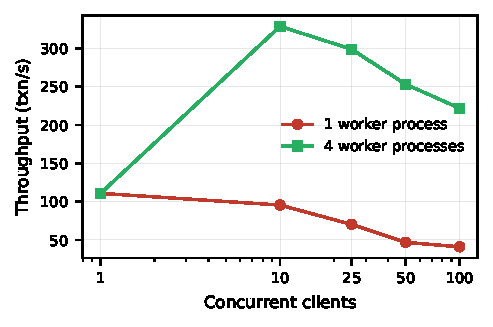
\includegraphics[width=\columnwidth]{figs/fig3_scaling.pdf}
\caption{Scoring-node throughput. A single process degrades under
concurrency (GIL contention); four worker processes restore near-linear
capacity, confirming the bottleneck lies in the stateless tier rather than
in the transactional ledger path.}
\label{fig:scaling}
\end{figure}

This is architecturally consequential. The design decision most exposed to
criticism --- holding row locks across a synchronous network call --- is
empirically not limiting at the concurrency levels examined, whereas the
limit resides in the one tier that is stateless and therefore trivially
replicable (Fig.~\ref{fig:scaling}). Interception correctness and scoring
capacity scale independently.

%==============================================================
\section{Deployment Recommendation}
\label{sec:deploy}

The experiments support a specific and actionable deployment posture, which
we state explicitly because the individual findings are otherwise easy to
read as merely diagnostic.

\textbf{Substitute the scorer.} LOF dominates the Isolation Forest on
detection at matched false-positive cost ($0.745$ vs.\ $0.147$) and on
inference latency ($1.67$\,ms vs.\ $5.46$\,ms). The interception
architecture is unchanged by the substitution: the scoring node's contract
is a feature vector in, a calibrated score out. This is a configuration
change, not a redesign.

\textbf{Replicate the scoring tier, not the ledger tier.} The concurrency
study localises the throughput constraint in the stateless inference node.
Capacity planning should provision inference replicas against offered load;
the transactional ledger path required no modification to sustain the
concurrency levels examined.

\textbf{Do not deploy a single-threshold hard block.} The threshold sweep
shows that no single cut separates genuine from fraudulent traffic
acceptably, even for the stronger scorer. A graduated response --- step-up
authentication in an intermediate band, hard block only at extreme scores
--- is not merely a refinement but a requirement implied by the measured
separability.

\textbf{Add sequence-aware features before claiming velocity coverage.}
The negative control's survival across both scorers establishes that no
per-transaction model will close this gap.

%==============================================================
\section{Limitations and Future Work}
\label{sec:limits}

\textbf{Archetype-design bias.} Three of the four archetypes (A, C, and to a
lesser extent D) manipulate transaction amount, so the injected set is
partially amount-separable by construction. This favours amount-sensitive
scorers in \emph{ranking} metrics --- an effect we observed directly, and
which underlies the anomalously high AUC of any amount-dominated score on
this set. It does not affect the operating-point comparisons, which are
budget-matched, but a fuller evaluation would include archetypes defined
solely by categorical or temporal deviation with amounts drawn from the
clean marginal.

\textbf{Population-level modelling.} The detector encodes what is anomalous
for the population, not for the individual account. A customer routinely
transferring large sums is indistinguishable from a compromised account
draining for the first time. Per-account rolling baselines --- deviation
from historical amount distribution, novel-payee and novel-device
indicators --- are the highest-value feature additions and are computable
from the existing audit table.

\textbf{Velocity blindness (measured).} The negative control quantifies a
hard boundary: zero detection of rapid-drain sequences. Windowed velocity
features over one-minute and one-hour horizons require a single indexed
query at enrichment time and a model retrain.

\textbf{Model selection.} The baseline study identifies LOF as dominant at
equal FPR under this encoding. A two-tier arrangement --- inexpensive forest
prefilter, density-based confirmation --- and target encoding of
categoricals to relieve one-hot dilution are the indicated next steps.

\textbf{Graduated friction.} The prototype hard-blocks and locks at
$\tau \geq 0.85$. At the measured $0.86\%$ false-positive rate, such a
posture applied at national scale would immobilise a substantial number of
legitimate accounts daily. A production design would introduce step-up
authentication in an intermediate band, reserve hard blocks for extreme
scores, and release locks through a support workflow rather than
permanently.

\textbf{Fail-closed availability.} Scoring unavailability currently rejects
all payments. A degraded-mode local rule engine behind circuit-breaker
semantics would bound the availability cost of the safety preference.

\textbf{Telemetry trust boundary.} Client-originated features remain
spoofable. The design mitigates but does not eliminate this, since plausible
spoofing shifts a transaction toward rarer, higher-scoring contexts.
Server-side verification of IP-derived geolocation would strengthen the
boundary.

\textbf{Prototype security scope.} MPIN digests use unsalted SHA-256 rather
than a memory-hard key-derivation function; transport is unencrypted; there
is no session authentication. These were excluded deliberately to isolate
latency measurement and are prerequisites for deployment.

\textbf{Measurement scope.} All figures are single-host and
loopback-networked, excluding datacenter latency, TLS termination, and
multi-tenant interference. Isolated ${\approx}4$\,s p99 outliers at burst
onset, attributed to JVM JIT warm-up and non-pooled harness connections,
are reported unfiltered and warrant elimination before publication-grade
tail-latency claims.

%==============================================================
\section{Conclusion}

We presented RT-IIPF, a working prototype relocating the payment-fraud
decision inside the transaction boundary, such that a rejected transfer is
rolled back atomically and never durably exists, while the security response
survives that rollback via an independent transaction.

Evaluation under synthetic fraud injection --- adopted because the public
corpus's labels proved uninformative --- produced findings we report
irrespective of their favourability, and their aggregate shape is
instructive. Two of the three deficiencies initially attributable to the
system proved not to be properties of the architecture at all. The
detection deficit dissolved under scorer substitution, recall rising from
$0.147$ to $0.745$ at unchanged operational cost and reduced latency. The
anticipated scaling ceiling proved to lie not in the lock-holding ledger
path we expected to indict, but in a stateless tier that replication
resolves. What remained after both corrections was a single genuine
architectural boundary: the velocity blind spot, which survived every
substitution and which no per-transaction scorer can close.

The methodological lesson generalises beyond this system. Each of these
conclusions required an experiment designed to be capable of embarrassing
the design --- a negative control, a budget-matched baseline, a contention
regime intended to expose lock serialisation. Evaluations constructed only
to demonstrate a system's strengths would have reported none of them, and
would have recommended the wrong remedy for two of the three problems.
Inline interception is a sound and model-agnostic mechanism; establishing
which of its limitations are architectural and which are incidental is the
work that makes it deployable.

\section*{Reproducibility}

Source, the evaluation harness, and the concurrency benchmark are available
at \todo{repository URL}. All experiments use seed~42.

% Entries [1]-[6] verified against publisher records (DOIs confirmed).
\begin{thebibliography}{00}
\bibitem{liu2008} F.~T. Liu, K.~M. Ting, and Z.-H. Zhou, ``Isolation
forest,'' in \emph{Proc. 8th IEEE Int. Conf. Data Mining (ICDM)}, Pisa,
Italy, Dec. 2008, pp.~413--422, doi: 10.1109/ICDM.2008.17.

\bibitem{breunig2000} M.~M. Breunig, H.-P. Kriegel, R.~T. Ng, and
J.~Sander, ``LOF: Identifying density-based local outliers,'' in \emph{Proc.
ACM SIGMOD Int. Conf. Management of Data}, Dallas, TX, USA, May 2000,
pp.~93--104, doi: 10.1145/342009.335388.

\bibitem{scholkopf2001} B.~Sch\"{o}lkopf, J.~C. Platt, J.~Shawe-Taylor,
A.~J. Smola, and R.~C. Williamson, ``Estimating the support of a
high-dimensional distribution,'' \emph{Neural Computation}, vol.~13,
no.~7, pp.~1443--1471, 2001, doi: 10.1162/089976601750264965.

\bibitem{campos2016} G.~O. Campos \emph{et al.}, ``On the evaluation of
unsupervised outlier detection: measures, datasets, and an empirical
study,'' \emph{Data Mining and Knowledge Discovery}, vol.~30, no.~4,
pp.~891--927, 2016, doi: 10.1007/s10618-015-0444-8.

\bibitem{abdallah2016} A.~Abdallah, M.~A. Maarof, and A.~Zainal, ``Fraud
detection system: A survey,'' \emph{Journal of Network and Computer
Applications}, vol.~68, pp.~90--113, 2016,
doi: 10.1016/j.jnca.2016.04.007.

\bibitem{adewumi2017} A.~O. Adewumi and A.~A. Akinyelu, ``A survey of
machine-learning and nature-inspired based credit card fraud detection
techniques,'' \emph{Int. J. System Assurance Engineering and Management},
vol.~8, no.~2, pp.~937--953, 2017, doi: 10.1007/s13198-016-0551-y.

\todo{Add 2--4 UPI-specific or Indian real-time-payment security
references to strengthen venue fit.}
\end{thebibliography}

\end{document}
